% File acl2014.tex
%
% Contact: koller@ling.uni-potsdam.de, yusuke@nii.ac.jp
%%
%% Based on the style files for ACL-2013, which were, in turn,
%% Based on the style files for ACL-2012, which were, in turn,
%% based on the style files for ACL-2011, which were, in turn, 
%% based on the style files for ACL-2010, which were, in turn, 
%% based on the style files for ACL-IJCNLP-2009, which were, in turn,
%% based on the style files for EACL-2009 and IJCNLP-2008...

%% Based on the style files for EACL 2006 by 
%%e.agirre@ehu.es or Sergi.Balari@uab.es
%% and that of ACL 08 by Joakim Nivre and Noah Smith

\documentclass[11pt]{article}
\usepackage{acl2014}
\usepackage{times}
\usepackage{url}
\usepackage{latexsym}
\usepackage{graphicx}


% My Package Includes
\usepackage{upquote} % For real apostrophes (see http://tex.stackexchange.com/questions/63345/how-to-make-a-real-apostrophe-or-single-quote-in-latex#63348)
\usepackage{comment}
\usepackage{xcolor}
\definecolor{dark-blue}{rgb}{0.15,0.15,0.7}
\usepackage{hyperref}
%\hypersetup{colorlinks, linkcolor={dark-blue}, citecolor={dark-blue}, urlcolor={dark-blue}}
\hypersetup{colorlinks, linkcolor=black, citecolor=black, urlcolor=black}
\usepackage{booktabs}
\frenchspacing % Normal (single) spaces after periods.  Cf. http://www.read.seas.harvard.edu/~kohler/latex.html
%\usepackage{natbib}
\usepackage[shortcuts]{extdash} % use "\-/" to help LaTeX insert hyphen/pagebreaks
\usepackage[textwidth=0.9in]{todonotes}
\newcommand{\smalltodo}[2][]
    {\todo[caption={#2}, #1]
    {\tiny#2\normalsize}}

% Have \autoref use the special section symbol instead of `section'.
\renewcommand{\sectionautorefname}{\S}
\renewcommand{\subsectionautorefname}{\S}
\renewcommand{\subsubsectionautorefname}{\S}

\newtheorem{requirement}{Requirement}

% GLOSSARIES PACKAGE
\usepackage{glossaries}
\glossarystyle{tree}
\makeglossaries
% commands to run to build the glossaries and acronyms files:
% makeindex -s computel_2014.ist -o computel_2014.gls computel_2014.glo
% makeindex -t computel_2014.alg -s computel_2014.ist -o computel_2014.acr computel_2014.acn

% End My Package Includes

\newacronym{api}{API}{application programming interface}
\newacronym{http}{HTTP}{Hypertext Transfer Protocol}
\newacronym{gui}{GUI}{graphical user interface}
\newacronym{ui}{UI}{user interface}
\newacronym{cl}{CL}{computational linguistics}
\newacronym{nlp}{NLP}{Natural Language Processing}
\newacronym{sil}{SIL}{Summer Institute of Linguistics}
\newacronym{json}{JSON}{JavaScript Object Notation}
\newacronym{npm}{NPM}{Node Package Manager}
\newacronym{bdd}{BDD}{behavior-driven development}
\newacronym{scrud}{SCRUD}{search, create, read, update, and delete}
\newacronym{rdbms}{RDBMS}{relational database management system}
\newacronym{igt}{IGT}{interlinear glossed text}
\newacronym{fst}{FST}{finite-state transducer}
\newacronym{cs}{CS}{context-sensitive}
\newacronym{lm}{LM}{language model}
\newacronym{url}{URL}{uniform resource locator}
\newacronym{tsv}{TSV}{tab-separated values}
\newacronym{tlg}{TLG}{Teach and Learn with Georgia}
\newacronym{flex}{FLEx}{FieldWorks Language Explorer}

%\setlength\titlebox{5cm}

% You can expand the titlebox if you need extra space
% to show all the authors. Please do not make the titlebox
% smaller than 5cm (the original size); we will check this
% in the camera-ready version and ask you to change it back.


\title{LingSync \& the Online Linguistic Database:\\New models for the
    collection and management of data for language communities, linguists and
language learners}

\author{Joel Dunham \\
University of British Columbia,   \\
Department of Linguistics \\
{\tt jrwdunham@gmail.com} \\\And
Gina Chiodo \\
iLanguage Lab \\
Montr\'eal \\
{\tt gina.chiodo@gmail.com} \\  \\\And
Joshua Horner \\
Amilia  \\
Montr\'eal \\
{\tt ~josh.horner@gmail.com} \\ }

%\author{First Author \\
%  Affiliation / Address line 1 \\
%  Affiliation / Address line 2 \\
%  Affiliation / Address line 3 \\
%  {\tt email@domain} \\\And
%  Second Author \\
%  Affiliation / Address line 1 \\
%  Affiliation / Address line 2 \\
%  Affiliation / Address line 3 \\
%  {\tt email@domain} \\}

\date{}

\begin{document}
\maketitle
%\tableofcontents

\begin{abstract}
LingSync and the Online Linguistic Database (OLD) are new models for the
collection and management of data in endangered language settings. The
Ling\-/Sync and OLD projects seek to close a feedback loop  between field
linguists, language communities, software developers, and computational
linguists by creating web services and \glspl{ui} which facilitate
collaborative and inclusive language documentation. This paper presents the
architecture of these tools and the resources generated thus far. We also
briefly discuss the integration of specific computational methods into the
systems, including the McGill Prosodylab-Aligner which provides automatic audio
alignment of novel data, as well as opportunities for research in
semi-unsupervised Machine Learning of language-independent morphological
analysis, and symbolic language-dependent analyzers. The paper discusses the
requirements of software used for endangered language documentation, and
presents novel data which demonstrates that users are actively seeking
alternatives despite existing software.
\end{abstract}


\section{Introduction}

In this paper we argue that the LingSync/OLD project forms a sustainable new
model for data management which facilitates a feedback loop between
fieldworkers, language communities, computational linguists and software
developers to maximize the results of language documentation efforts for
low-resource language communities. In \autoref{sec:requirements} we present
five requirements for endangered languages fieldwork software  which are
currently not met by existing language documentation software discussed in
\autoref{sec:existing-software}. Architectural considerations%
\footnote{For further discussion of actual user interaction, screenshots and
    how LingSync/OLD data can be exported/published in existing online
    linguistics repositories such as EOPAS \url{http://www.eopas.org/} and OLAC
    \url{http://www.language-archives.org/} see \cite{lingsync:2012}.} %
under LingSync and the OLD which address these requirements are briefly
outlined in \autoref{sec:lingsync-old}.  The ability of LingSync/OLD to
integrate with existing software libraries commonly used in language
documentation projects is demonstrated in \autoref{sec:plugins}. Finally,
\autoref{open-data} demonstrates how the LingSync/OLD project is already
seeing some closure of the feedback loop both in creating language learning
apps for heritage speakers and in training Kartuli speakers to build speech
recognition systems built on LingSync/OLD data.


%%%%%%%%%%%%%%%%%%%%%%%%%%%%%%%%%%%%%%%%%%%%%%%%%%%%%%%%%%%%%%%%%%%%%%%%%%%%%%%%
% Endangered Languages fieldwork
%%%%%%%%%%%%%%%%%%%%%%%%%%%%%%%%%%%%%%%%%%%%%%%%%%%%%%%%%%%%%%%%%%%%%%%%%%%%%%%%

\section{Endangered languages fieldwork}\label{sec:fieldwork}

Endangered languages are valuable culturally and scientifically, to their
communities of origin \cite{Ironstrack:2012} and to humanity as a whole
\cite{harrison2007languages}. Efforts must be made to document these languages
while there is still time \cite{Good:2012,Thieberger:2012}. 
%The communities
%from which endangered languages originate, while also valuing documentation,
%are equally interested in increasing the rates at which their languages are
%transmitted and used \cite{Myaamia:2001}. 
In cases where there are no longer
any native speakers, a community may embark upon a language reclamation project
that is wholly dependent upon the the products of past language documentation
efforts \cite{Leonard:2012,Costa:2012}. Alongside such documentation and
revitalization/reclamation projects is research-driven linguistic fieldwork.
These diversely motivated yet interconnected strands within endangered
languages fieldwork conspire to produce a particular set of requirements for
effective software in this domain.


\subsection{Software requirements}
\label{sec:requirements}

Though often overlooked, we claim that the following five requirements are
essential to effective language documentation software: \emph{Integration of
primary data}, \emph{curation of data}, \emph{inclusion of stakeholders},
\emph{openable data}, and \emph{user productivity}.


\begin{requirement}
	\label{req:primary-data}
       Integration of primary data
\end{requirement}

While language reclamation projects founded solely on textual data can achieve
some degree of success \cite{Ironstrack:2012}, primary audio/video data \emph{in the
form of engaging content} is crucial to fostering native-like proficiency.
Primary audio has formed part of language documentation efforts since
the days of phonographs, yet only rarely have such audio products
been made accessible. Securely and efficiently supporting the integration of
primary audio/video data with text artifacts (e.g., dictionaries, grammars,
collections of narratives) is part of the requirements of any modern language
documentation effort \cite{Schroeter:2006,Good:2012b}.%
\footnote{For a more detailed discussion of the technical limitations which are
    no longer blocking the implementation of these requirements see
\cite{lingsync:2012}.}


\begin{requirement}
	\label{req:curation}
       Curation of data
\end{requirement}

While most language documentation literature places emphasis on the creation of
artifacts, our experience has shown that a significant percentage of language
documentation hours are actually dedicated to the curation and filtering of the
data in preparation for publication as artifacts.%
\footnote{Such artifacts might include engaging content to be reused in
    revitalization efforts, or citable/traceable data sets used to support
research claims.}
Even ``a funding body like the ELDP cannot get all of its grantees [only 110
out of 216] to deposit in an archive in a timely fashion (or at all)''
\cite{Thieberger:2012}. We argue that
facilitating the collaborative curation of data is, in fact, a core requirement
of any data management or content management software, one which is largely
overlooked by existing software (cf.
\autoref{sec:existing-software}).


\begin{requirement}
	\label{req:inclusive}
       Inclusion of stakeholders
\end{requirement}

A sustainable language documentation effort involves crucially the creation of a
positive feedback loop where the outputs of certain activities fuel
the advancement of others.
%For example, linguistic research generates data that can benefit the
%revitalization and reclamation efforts of language communities; Computational
%linguistics research on low-resource languages benefits software libraries,
%software developers use libraries which do not break content in low-resource
%languages, and increased language community presence on the web, results in
%more accessible primary data, which is a benefit to both linguistic and
%computational linguistic research.
However, realizing this feedback loop requires tools that facilitate the
inclusion of the various stakeholders involved in the process of language
documentation \emph{while} a project is underway, not \emph{post hoc} when
the data is ``polished,'' which in 50\% of projects never happens
\cite{Thieberger:2012}. This inclusivity requirement means that data and data
processes must be available in formats that are usable to both humans---i.e.,
via \glspl{gui}---and machines---i.e., via software libraries and \glspl{api}.

% I COMMENTED THIS OUT BECAUSE IT IS NO LONGER OVERTLY REFERENCED IN THE PAPER ...
\begin{comment}
\begin{table}[h]
\begin{center}
\scriptsize
\begin{tabular}{llll}
      \toprule
      Stakeholders & Default Context & Mobile Context\\\hline\hline
     
      Language Community & Windows &  iPhone, Android\\
      \midrule

	Field Linguists & Mac, Windows, Linux & iPad, Android\\
	  & Praat, Javascript, LaTeX \\
	  \midrule

	Computational Linguists & Linux, Mac, Windows\\
	 & GATE, UIMA, Pip, NLTK\\
	\midrule

	Web Developers & Mac, Linux, Windows\\
	 & Brew, NPM\\

      \bottomrule

\end{tabular}
\caption{Contexts both in terms of operating systems and programming languages/frameworks where data and  data processes must be available.}
\label{requirements-contexts}
 \end{center}
 \normalsize
\end{table}
\end{comment}
% END COMMENT


\begin{requirement}
	\label{req:openable}
       Openable data
\end{requirement}

One of the unique challenges associated with endangered languages fieldwork is
the possibility that speakers or language communities may require that all or
aspects of the raw data be kept confidential for a certain period of time.%
\footnote{Outside of language documentation contexts there are numerous valid
    reasons for facilitating data privacy. As with social websites
    (Facebook, YouTube), user data is generally considered private and not
    accessible to data scientists. Many content curation sites (Google Docs,
    WordPress) allow for content that is private indefinitely or during a
pre-publication stage.} %
Labs looking to reuse the data collected by field teams may, in particular, be
unaware of the post-colonial context in which many fieldwork situations are
embedded.

In the field it often happens that a speaker will speak quite candidly or
receive a phone call  during a recorded elicitation session and may want to
restrict access to all or parts of that recording for personal reasons.% 
\footnote{Of course, as one reviewer points out, basing claims on private data
    runs contrary to a core tenet of the scientific method, namely that claims
    must be able to be assessed with transparent access to the methods and data
    used to support them.  However, in these contexts field linguists generally
    protect the privacy of their language consultants by eliciting novel
    sentences which have similar grammatical features for publication, rather
    than using the original narrative. In the contexts of open data, such
    highly personal sections of transcripts must be ``blacked out'' so that the
majority of the data can be made open.} %
In some cases the living speakers of the language are so few that even
anonymizing the data does not conceal the identity of the speaker from other
speakers in the community.  It also happens that particular stories or
descriptions of rituals and cultural practices may need to be restricted to just
the language community or even to sub-groups within the community.%
\footnote{It is highly preferable for language communities to produce
their own content using YouTube and other content sites, permitting the
community to manage censorship of sensitive topics and personal narratives
while creating more public data.}

In order to provide access to all team members and stakeholders (including
stakeholders who are distrustful of the project) language documentation
software must support a non-trivial permissions system while also facilitating
transparency and encouraging open collaboration. Even language documentation
projects using ad hoc content creation solutions (discussed in
\autoref{sec:existing-software}) cannot be fully inclusive for fear that when
speakers of different dialects disagree they will ``correct''  each other's
data if neither social pressure nor the permissions system prevents it.
In fact, disagreements about data judgments remain an untapped indirect source
of grammaticality information for linguistics researchers as there are no
language documentation systems which permit inclusion of all stakeholders via
traceable user activity, non-trivial permissions systems, and confidentiality
of attributes on data. While not all teams will resort to data encryption or
private data, implementing these features permits more stakeholders to have
direct conditional access to data and removes barriers to adoption by language
communities who may be initially distrustful of language documentation
projects.%

%\smalltodo{we let teams decide what to do in these cases, do they think they
%can use social pressure to prevent data correction, or do they need to teach
%some users how to password protect their data, or put their data in different
%databases or... we make the tools so the teams can do what they want.}



\begin{requirement}
	\label{req:productivity}
       User productivity
\end{requirement}

Users are accustomed to professionally crafted software built by teams
of hundreds of software engineers, software designers, and user experience
experts (e.g., Facebook, Gmail, Google Docs, YouTube, Evernote, Dropbox). They
can read their email on all devices, download and sync photos and videos
automatically, and have offline and mobile data there seamlessly when they need
it. Yet research software is often built by computer science students with no
experience in software engineering and human computer interaction.
Overwhelmingly, users attribute their use of generic data curation software
such as Microsoft Excel or Google Spreadsheets, rather than software
specifically designed for language documentation, to the productivity of the
user experience itself \cite{lingsync:2012}. In some cases users are so
productive using Google Spreadsheets that the actual data entry of a project
can be completed before an existing language documentation tool can be
evaluated and/or customized \cite{Troy:2014}.


\subsection{Existing software}
\label{sec:existing-software}

Fieldwork teams typically have the choice between using general-purpose content
curation software (Google Spreadsheets, Evernote, Dropbox, MediaWikis,
WordPress etc.), creating/customizing their own tools, or using specialized
field linguistics desktop applications such as those developed by SIL
International: \gls{flex},%
\footnote{ \url{http://fieldworks.sil.org/flex} } %
 Toolbox/Shoebox,%
\footnote{Toolbox is the community-supported continuation of Shoebox
\url{http://www-01.sil.org/computing/toolbox/information.htm}} %
and/or WeSay.%
\footnote{\url{http://www.sil.org/resources/software\_fonts/wesay}}

The SIL tools%
\footnote{For reviews of \gls{flex} and Toolbox, see
\cite{Butler:2007,rogers10,robinson07}.} %
require a not inconsiderable level of training in order to be used productively.
However, many research teams are unable to impose lengthy training upon all
team members and require tools that are easy to learn and re-learn months or
years later when they return to their data. In addition, the SIL tools are
tailored towards the collection of texts and the production of dictionaries and
descriptive grammars based on such. However, this focus does not always accord
with the needs of research-oriented fieldworkers, many of whom deal primarily
in sentences elicited in isolation and grammaticality judgments.
%In order to maximize productivity (Req.  \autoref{req:productivity}), tools
%must be easy to learn and re-learn months or years later when users return to
%their data.

%The SIL tools were developed primarily with practical lexicography in mind, and
%as such are not ideally suited to research teams which spend only a percentage
%%of their hours interacting with data management software. Unlike professional
%lexicography teams, most research teams are unable to impose lengthy tool
%training upon all team members; to maximize productivity (Req.
%\autoref{req:productivity}) tools must be easy to learn and re-learn months or
%years later when users return to their data.

Existing language documentation software tools, with the exception of WeSay (a
collaborative dictionary tool), have only ad hoc support for collaboration
(Req. \autoref{req:openable}) and inclusive language documentation (Req.
\autoref{req:inclusive}) while the project is active, generally using a shared
network drive or email with no concurrent editing. \gls{flex} and many private
tools in the language technology industry are able to support concurrent
editing in most data entry situations via a Mercurial/SVN/CVS/Git repository
\cite{FLExSendReceive:2013:Online}. 
% The benefit of using a full-fledged version control
%system is that the history of the data is viewable.  
However, as no permissions are built into Mercurial/SVN/CVS/Git, users with
read only access  must use a manual review process to offer their modifications
to the project. 
%While FLEx does support
%collaboration, the support for collaboration requires a small degree of
%technical understanding from all team members to avoid merge conflicts.  
The \gls{flex} Send/Receive  collaboration module also limits the integration of
audio/video primary data; it unfortunately does not support formats used by
field linguists including .ogg, .avi, .mp4, and .mov, and limits the maximum
file size to 1MB  \cite{FLExSendReceive:2013:Online}, despite the fact that
most elicitation sessions or long utterances can range between 10MB and 200MB. 
While these scenarios may seem like rare edge cases, they can, in fact, result
in teams opting not to use software designed for language documentation.

%For research teams, the primary artifacts
%generated are not dictionary entries but rather sentences and grammaticality
%judgments. 

Over the past decade or so, a number of language-specific collaborative
websites have arisen, examples of which are the Yurok Documentation Project
\cite{Yurok:2001:Online}, the Washo Project
\cite{Washo:2005:Online,Cihlar:2008}, the Washo Mobile Lexicon
\cite{WashoMobile:2008:Online}, Karuk Dictionary and Texts
\cite{Karuk:2009:Online}, and the Ilaatawaakani project \cite{Troy:2014}. More
recently, collaborative  tools have arisen that, like \gls{flex} and Toolbox, are not
specific to any one language, but unlike \gls{flex} and Toolbox, run on all devices
in a web browser.  In this family belong TypeCraft \cite{Beermann:2012}, the
OLD \cite{dunham2014docs}, and LingSync \cite{lingsync:2012}.

TypeCraft uses a MediaWiki \gls{ui} combined with additional functionality
written in Java for managing collaboration permissions and sharing. TypeCraft
falls into the category of field databases designed by corpus linguists. As
such it imposes upon users closed lists of categories for languages and parts
of speech \cite{Farrar:2010}, an imposition which is unacceptable to field
linguists who are dealing with evolving fine-grained analyses of data
categories. In addition, TypeCraft is online only, a limitation which, as
Farrar correctly points out, is ``not inconsiderable, especially for
fieldworkers who may not have Internet access'' \cite{Farrar:2010}.

None of the software projects discussed in this section meet the software
requirements for endangered languages fieldwork outlined in
\autoref{sec:requirements}. We argue that this mismatch in requirements is
non-trivial and is the reason why so much fragmentation and introduction of novel
language documentation tools and software has occurred.%
\footnote{We would like to point out that there are numerous other projects
    that have started and failed in the past 10 years which we have not had
    space to mention. The only stable long-term fieldwork software projects
    have been those which have been undertaken by the \gls{sil}. The SIL
    development team is also on GitHub (\url{https://github.com/sillsdev}), a
    social tool for open source project management; this will likely yield
    technical crossover with research teams and more use of HTML5 to facilitate
    meeting the requirements delineated in \autoref{sec:requirements} in future
SIL software.} %



\section{New models for data collection and management}
\label{sec:lingsync-old}


\subsection{LingSync}\label{sec:lingsync}

%LingSync is an open source project which began on April 20th 2012. 
LingSync is
composed of existing and novel open source software modules (rich client-side
web components and task-specific web services) which allow all stakeholders of
a language documentation effort to collaboratively create corpora of primary
analyzed and unanalyzed language data \cite{lingsync:2012}.

To meet the user productivity requirement (Req. \autoref{req:productivity}),
LingSync uses a quasi-blackboard system architecture similar to
Android;\footnote{\url{http://developer.android.com}} that is, modules can be
registered to perform certain tasks, and users can discover and choose between
registered modules. Similar to Praat,%
\footnote{\url{http://praat.org}} %
all events in the system provide an audit trail which can be used by users,%
\footnote{In the case of Praat users are able to generate automation scripts by
clicking to create a repeatable sequence of events.}
but also serve as data for automated reasoning engines, should labs choose to
make use of the audit data to assist in data cleaning (Requirement
\autoref{req:productivity}) and data quality (Requirement
\autoref{req:openable}).

%LingSync introduces novel data about the data collection process itself. 
Based on the LingSync team's collective prior experience as field linguists,
research assistants, professional lexicographers, and linguists in the language
technologies industry, we hypothesize that perhaps 50\% of data
curation/cleaning tasks are monotonous, repetitive and consistent and thus are
candidates for data manipulation best done by machines or crowdsourcing rather
than by one individual human for extended periods of time.  The automation of
tasks in field linguistic research is rarely done, and for good reason. Unlike
corpus linguistics, field linguistics seeks fine-grained analysis of novel data
on undocumented languages, and data curators must be sensitive to the slightest
``off'' feeling of analysis which could easily be flattened by
over-generalizing cleaning scripts.  Automated modifications must be fully
traceable in their motivations so as to detect side effects of cleaning long
after it has occurred. They must also be easily undoable so as not to introduce
consistency or systematicity which in fact does not exist in the data.
%To better identify the role of machines in data cleaning in
%a language documentation context, LingSync's implementation collects the data
%required to more accurately identify the ratio of tasks best done by machine to
%tasks best done by humans. 

The potential time-saving features of Ling\-/Sync's system design will not bear
usable data without the explicit and overarching goal of providing a
user-friendly experience for both expert and novice users with differing data
description vocabularies and interests \cite{Troy:2014}.  Notable user-facing
features include complete \gls{ui} customization, powerful searches and mapping over
data sets, encryption at a field level, flexible enforcement of data
consistency, social collaborative software features, an inclusive permissions
system, pluggable 
semi-automatic glossers, numerous task-oriented web services which wrap
existing libraries and scripts for audio, video, image and text analysis, two
native Android \glspl{gui} which function offline (Learn X and the Elicitation
Session Recorder), and five browser-based \glspl{gui} (the Prototype,
Spreadsheet,  Activity Feeds, Corpus Pages, Lexicon Browser), one of which
functions offline and provides flexible import and export functionality. 
%
%LingSync's libraries and components are built entirely using HTML5 technologies
%and current best practices for rich JavaScript client-side apps including
%\gls{bdd} testing, and build and dependency management frameworks analogous to
%Java's JUnit, Gradle and Maven.%
%\footnote{As of 2014 these are Jasmine (testing), Grunt (build automation), and
%    \gls{npm} (dependency management):\\
%    \url{http://jasmine.github.io}, \\
%    \url{http://gruntjs.com}, \\
%\url{https://npmjs.org}}
%Data is stored in \gls{json} using Apache CouchDB%
%\footnote{\url{http://couchdb.apache.org/}} %
%on the server-side (permitting scalable, decentralized, and fully replicated
%data stores) and IndexedDB on the client-side. 
%
Nearly all logic is performed on
the client-side which permits users to go offline and consume low bandwidth
when there is limited connectivity through 3G or dial-up connections.
%
For up-to-date examples of \gls{gui} interaction, readers are encouraged to
search for LingSync on YouTube. As of April 2014 there are over 40 videos made
by users demonstrating diverse features in the systems.



\subsection{OLD}\label{sec:old}

The OLD is software for creating web services that facilitate collaborative
linguistic fieldwork. A language-specific OLD web service exposes a consistent
\gls{api},%
\footnote{The OLD \gls{api} is RESTful and \gls{json} is used as the medium
    of exchange throughout. This means that OLD resources (e.g., linguistic
    data points such as sentences) can be created, retrieved, updated, deleted,
    and searched using standard combinations of \gls{http} methods and \gls{url}
    patterns. The system is written in Python using the Pylons web framework
    (\url{http://www.pylonsproject.org/projects/pylons-framework/about}) and the
relational database software MySQL.} %
meaning that it can easily be used as the backend to multiple user-facing
applications or as a component in a larger suite of tools. An OLD web service
and the current OLD \gls{gui} together provide a number of features that
respond to the requirements given in \autoref{sec:requirements}.

A language-specific OLD application allows for multiple contributors to
simultaneously create, modify, browse, and search language data. This data
consists of linguistic forms (i.e., morphemes, words, or phrases) that can be
used to build corpora and texts. The OLD supports the integration of primary
audio/video data by allowing for individual forms to be associated to any
number of audio or video files (or even to subintervals of such files) and
by generating representations wherein textual and audio/video data are
simultaneously accessible. Data is presented in \gls{igt} format and individual
forms, collections of forms, and texts can be exported as (Xe)LaTeX, \gls{tsv},
or plain text. The system provides powerful search functionality including filters
over system-generated serializations of morphological analyses and, via integration
with TGrep2,%
\footnote{\url{http://tedlab.mit.edu/~dr/Tgrep2/}.} %
the matching of structural patterns within treebank corpora.

Features promoting consistency include configurable orthography converters,
inventory-based input validation, and the provision of visual feedback on
the extent to which user-generated morphological analyses match existing
lexical entries in the database. That last feature means that when a user
creates a morphologically complex entry, the \gls{igt} representation
indicates, via colour-coded internal links, whether the morpheme shapes and
glosses match current lexical entries. It has proved to be quite useful in
helping groups of fieldworkers to generate consistent morphological analyses.


\subsection{LingSync/OLD}

While LingSync and the OLD arose independently and consequently use different
technology stacks, the teams behind the tools have largely complementary
interests and are collaborating on future developments in order to combine
strengths and reduce fragmentation of efforts. In the coming years, if resources
permit, we hope to bring OLD's glossing \glspl{ui}, logic for connecting
documents to utterances as well as structural search and morphological parsing
(\autoref{sec:old-parsers}) into the LingSync plugin architecture, with OLD
\glspl{ui} being used by field linguists and LingSync \glspl{ui} being used by
language community members and computational linguists. When referring
collectively to both tools, we will henceforth use the term LingSync/OLD.


\section{User adoption}

In the year and a half since LingSync's launch, over 300 unique users have
registered; this despite the availability of a sample user (username:
LingLlama, password: phoneme). We argue this demonstrates a general interest in
novel, even unheard-of, language documentation software, despite the existing
solutions discussed in \autoref{sec:existing-software}.

\autoref{lingsync-data} provides an overview of the corpora being edited using
the system. Currently there are about 13,400 active records, 38 active users,
15 active corpora, and 1GB of primary audio/image/text data. We expect that the
low ratio of active vs. registered users (12\%) is due to both the multi-task
nature of language documentation projects and early launch of LingSync while it
was still in the alpha testing and the requirements gathering phase.  There are currently no published measures of user
attrition in language documentation projects, however social websites/mobile
apps  developers report 30\% retention rate is acceptable.%
\footnote{There are no official published statistics; however, in answers on
    StackOverflow developers report averages to be 30\%, cf.
http://stackoverflow.com/questions/6969191/what-is-a-good-active-installs-rate-for-a-free-android-app.}
We will
know more about rates for different stakeholders in language documentation projects as the retention rate changes over time  in correlation to the
release of new modules.

\begin{table}[h]
\begin{center}
\scriptsize
\begin{tabular}{lrrrr}
      \toprule
                     ~ &  Active & Investigating & In-active & Total\\
      \midrule
      Public Corpora  &       2 &   1 &   2 & 5 \\ 
      Private Corpora &      15 &  37 & 321 & 373\\ 
      Users           &      38 &  43 & 220 & 301 \\
      Documents & 13,408 & 2,763 & 4,541 &23,487\\
      Disk Size & 1GB & .9GB & 5.3GB& 7.2GB\\
      
      \bottomrule

\end{tabular}
\caption{Data in LingSync corpora (Feb 14, 2014). Active corpora: $>$300
activities; Investigating corpora: 300-10 activities; Active users: $>$100
activities; Investigating users: 100-10 activities.}
\label{lingsync-data}
 \end{center}
 \normalsize
\end{table}


There are currently nine language-specific OLD applications in use. In total,
there are about 19,000 records (primarily sentences), 300 texts, and 20 GB of
audio files.  There are 180 registered users across all applications, of which
98 have entered and 87 have elicited at least one record. The applications for
Blackfoot, Nata, Gitksan, Okanagan, and Tlingit are seeing the most use. The
exact figures are summarized in \autoref{old-data}.%
\footnote{ Note that the values in the speakers column are taken from
    Ethnologue (\url{http://www.ethnologue.com}) and are provided only to give
    a rough indication of the speaker populations of the languages. Also, the
    three-character codes in the first column are the ISO 639-3
(\url{http://www-01.sil.org/iso639-3}) identifiers of the languages.}


\begin{table}[h]
 \begin{center}
     \scriptsize
\begin{tabular}{lrrrrr}

      \toprule
      language &                     \emph{forms}  & texts & audio & GB   & speakers \\
      \midrule
      Blackfoot (\textit{bla}) &     8,847  & 171   & 2,057 & 3.8  & 3,350    \\ % 11,075 4047074461 bytes
      Nata (\textit{ntk}) &          3,219  & 32    & 0     & 0    & 36,000   \\ % 3,251  0 bytes
      Gitksan (\textit{git}) &       2,174  & 6     & 36    & 3.5  & 930      \\ % 2,216  3787227136 bytes
      Okanagan (\textit{oka}) &      1,798  & 39    & 87    & 0.3  & 770      \\ % 1,924  349478912 bytes
      Tlingit (\textit{tli}) &       1,521  & 32    & 107   & 12   & 630      \\ % 1,660  12906459136 bytes
      Plains Cree (\textit{crk}) &   686    & 10    & 0     & 0    & 260      \\ % 696    0 bytes
      Ktunaxa (\textit{kut}) &       467    & 33    & 112   & 0.2  & 106      \\ % 612    176128000 bytes
      Coeur d'Alene (\textit{crd}) & 377    & 0     & 199   & 0.0  & 2        \\ % 576    28659712 bytes
      Kwak'wala (\textit{kwk}) &     98     & 1     & 1     & 0.0  & 585      \\ % 100    7450624 bytes
      TOTAL &                        19,187 & 324   & 2,599 & 19.8 &         \\ % 22,110 21302477981 bytes
      \bottomrule

\end{tabular}
\caption{Data in OLD applications (Feb 14, 2014)}
\label{old-data}
 \end{center}
 \normalsize
\end{table}

The data in \autoref{lingsync-data} and \autoref{old-data} indicate that the
systems are in fact being used by language documentation teams. 



\section{Reusing existing tools and libraries}
\label{sec:plugins}


Both the LingSync and the OLD projects were founded with the goal of making it
easier to integrate existing software
libraries to better automate data curation (Req. \autoref{req:curation}) and 
improve data quality (Req. \autoref{req:openable}) while doing fieldwork. There have been numerous
plugins in both systems to this end; however in this paper we will discuss only
those which may be of most interest to computational linguists working on
low-resource languages: morphological parsers in \autoref{sec:farley}, 
\autoref{sec:old-parsers} and \autoref{sec:lingsync-glosser} which are a
precursor for Information Retrieval and Machine Translation tasks, and 
phone-level alignment of audio and text in \autoref{sec:aligner} which is a
precursor for acoustic model training in Speech Recognition systems.



\subsection{Existing morphological parsers}
\label{sec:farley}

For one LingSync team working on Inuktitut, a web service was written which
wraps an existing morphological analyzer for Inuktitut built in Java
\cite{Farley:2012:Online}. This source code can be used to wrap other existing
language-specific morphological analyzers.%
\footnote{All modules discussed in this paper are available by searching the
    GitHub organization page
\url{https://github.com/FieldDB}}


\subsection{Novel morphological parsers}
\label{sec:old-parsers}

An OLD web service provides functionality that allows users to create any
number of morphological parsers. The phonological mappings of these parsers
are declared explicitly, using a formalism---\gls{cs} phonological rewrite
rules \cite{chomsky68}---that is well understood by linguists. The lexicon,
morphotactic rules, and parse candidate disambiguator components are
automatically induced from corpora specified by the user. The fact that this
implementation requires a good deal of explicit specification by the user
should not be considered a demerit. By granting linguist fieldworkers control
over the specification of phonological, lexical, and morphotactic
generalizations, the parser functionality allows for the automatic testing of
these generalizations against large data sets. This assists in the discovery of
counterexamples to generalizations, thereby expediting the improvement of
models and advancing linguistic research. The OLD morphological parser
implementation can, of course, co-exist with and complement less
expert-dependent Machine Learning approaches to creating morphological parsers.

The core component of an OLD morphological parser is a morphophonology that is
modelled as a \gls{fst}%
\footnote{\glspl{fst} are constructed using the open source finite-state
compiler and C library foma: \url{http://code.google.com/p/foma}} %
and which maps transcriptions to morphological analyses, i.e., morpheme
segmentations, glosses, and categories. The morphophonology \gls{fst} is the
composition of a phonology \gls{fst} that is created explicitly by the user
(using \gls{cs} phonological rewrite rules) and a morphology (i.e., lexicon and
morphotactic rules) that is induced from corpora constructed by the user, cf. 
\cite{beesley2003finite,hulden2012}. When the morphophonology returns multiple
parse candidates, the system employs an $N$-gram \gls{lm}%
\footnote{OLD $N$-gram \glspl{lm} are estimated using MITLM:
\url{https://code.google.com/p/mitlm/}.} %
(estimated from a corpus specified by the parser's creator) to determine the
most probable parse.

Preliminary tests of the OLD morphological parser implementation have been
performed using data from the Blackfoot OLD%
\footnote{\url{http://bla.onlinelinguisticdatabase.org/}} %
and the standard grammar \cite{frantz91} and dictionary \cite{frantz95} of the
language. An initial parser implemented the phonology specified in
\cite{frantz91} and defined a morphology with lexical items extracted from
\cite{frantz95} and morphotactic rules induced from words analyzed by
contributors to the system. Analysis of the performance of this parser
(f-score: 0.21) confirms what researchers \cite{weber2013} have already
observed, namely that the phonological and morphological generalizations of
\cite{frantz91} cannot account for the location of morphologically conditioned
prominence (i.e., pitch accent) in Blackfoot words.

An improved Blackfoot parser, i.e., one which can predict prominence location
based on the generalizations of \cite{weber2013}, is currently under
development. The phonology of this parser makes use of a novel and useful
feature, viz. the ability to specify phonological transformations that are
aware of categorial context. This allows the phonology to capture the distinct
nominal and verbal prominence location generalizations of Blackfoot.

Since OLD morphological parsers can be created and parses retrieved entirely by
issuing RESTful requests, other applications can easily make use of them. In
addition, OLD morphological parser objects can be exported as .zip archives
that contain all of the requisite binaries (i.e., compiled foma and MITLM
files) and a Python module and executable which together allow for the parser
to be used locally via the command line or from within a Python program.



\subsection{Semi-supervised morphological parsers}
 \label{sec:lingsync-glosser} 

LingSync's glosser uses a MapReduce function which efficiently indexes and transforms data 
 to create a current ``mental lexicon'' of the corpus.  The
mental lexicon is modelled as a connected graph of morphemes, including
precedence relations which are used to seed finite-state automata \cite{Chiodo:2009}%
\footnote{One reviewer requests more details which have not yet been published:
    in the interim please consult the code which is entirely open source and
    commented:  \\
\url{https://github.com/FieldDB/FieldDBGlosser}} %
which represent morphological templates in the corpus. In this way the glosser
is ``trained'' on the user's existing segmentation and glossing, and
automatically ``learns'' as the user adds more data and the
glossing/segmentation evolves over the course of data collection and analysis. 
LingSync has a lexicon browser component which permits users to browse the
corpus via learned  relations between morphemes, clean the data for
consistency, enter novel data, and explicitly document generalizations on
lexical nodes which might not be immediately evident in the primary data. 
Unlike \gls{flex} \cite{Black:2006}, the OLD and WeSay, LingSync does not
provide a way to explicitly add rules/relations or morphemes which are not
gleaned from the data. To add a morpheme or a relation users must add an
example sentence to the corpus. This grounding of morphemes and rules/relations
provides arguably better learning tools as collocation dictionaries and
lexicon creators are always able to provide headwords and grammatical rules in
context and researchers working on relations between morphemes are able to
extract lists of relevant data.

\begin{figure}
\begin{center}
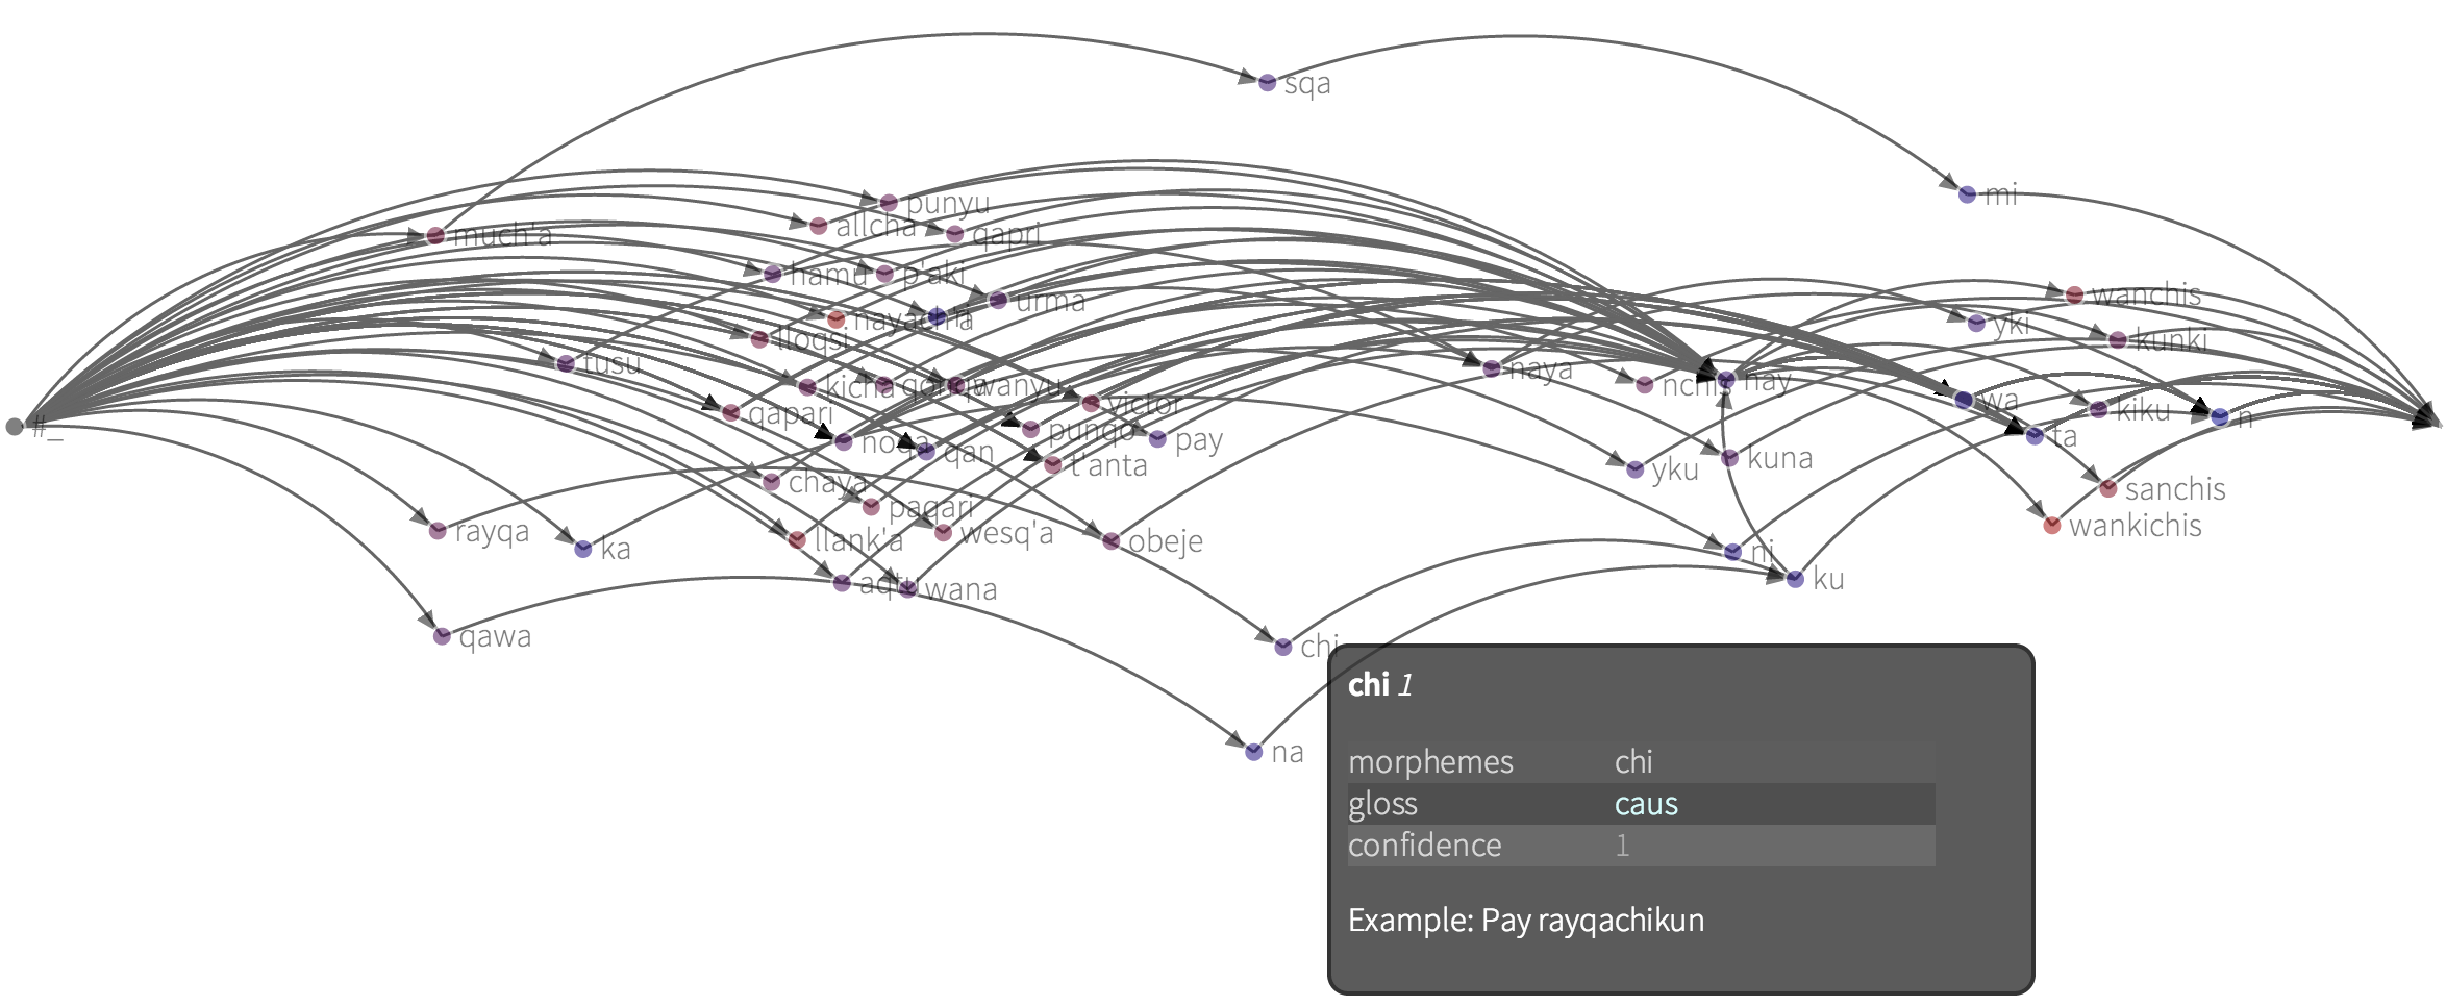
\includegraphics[width=3in]{images/lexicon_browser}
\caption{Screenshot of the Lexicon Browser, a web widget which lets users
browse relations between morphemes in their corpus, clean and add
declarative knowledge not found in the lexicon training process.}
\label{lexicon_browser_screenshot}
\end{center}
\end{figure}



\subsection{Audio-transcription alignment}
\label{sec:aligner}

There are currently three audio web services. The first executes Sphinx speech
recognition routines for languages with known language models. The second,
illustrated in \autoref{fig:api-audio}a, uses the Prosodylab-Aligner%
\footnote{\url{https://github.com/kylebgorman/Prosodylab-Aligner}} %
tool (developed at the McGill Prosody Lab) to significantly automate the
association of transcriptions to relevant audio clips and therefore help to
provide a class of data that will prove valuable in applications such as
talking dictionaries and language learning tools. The third, illustrated in
\autoref{fig:api-audio}b, is a service that wraps FFmpeg%
\footnote{\url{http://www.ffmpeg.org/}} %
and Praat%
\footnote{\url{http://www.praat.org/}} %
to convert any video or audio format to .mp3 and automatically generate
syllable timings and suggested utterance boundaries \cite{DeJong:2009} for
automatic chunking of data.


\begin{figure}[h]
\scriptsize
\begin{verbatim}
a) $ curl --cookie my-cookies.txt\
  --request POST\
  -F files[]=@omi_imitaa.mov\
  -F files[]=@omi_imitaa.lab\
  https://api.lingsync.org/v2/corpora/public-curldemo/
  utterances?process=align

b) $ curl --cookie my-cookies.txt\
  --request POST\
  -F files[]=@omi_imitaa.mov\
  https://api.lingsync.org/v2/corpora/public-curldemo/
  utterances?process=detect
  
c) $ curl --cookie my-cookies.txt\
  --request GET\
  https://api.lingsync.org/v2/corpora/public-curldemo/
  files/omi_imitaa.mp3
 
d) $ curl --cookie my-cookies.txt\
  --request GET\
  https://api.lingsync.org/v2/corpora/public-curldemo/
  files/omi_imitaa.TextGrid
   
\end{verbatim}
\caption{Audio/video and text alignment via Prosodylab-Aligner web service (a),
detecting utterances and syllable timing from audio/video files (b), retrieving
web playable audio (c), and TextGrid results (d).}
\normalsize
\label{fig:api-audio}
\end{figure}


\begin{figure}
\begin{center}
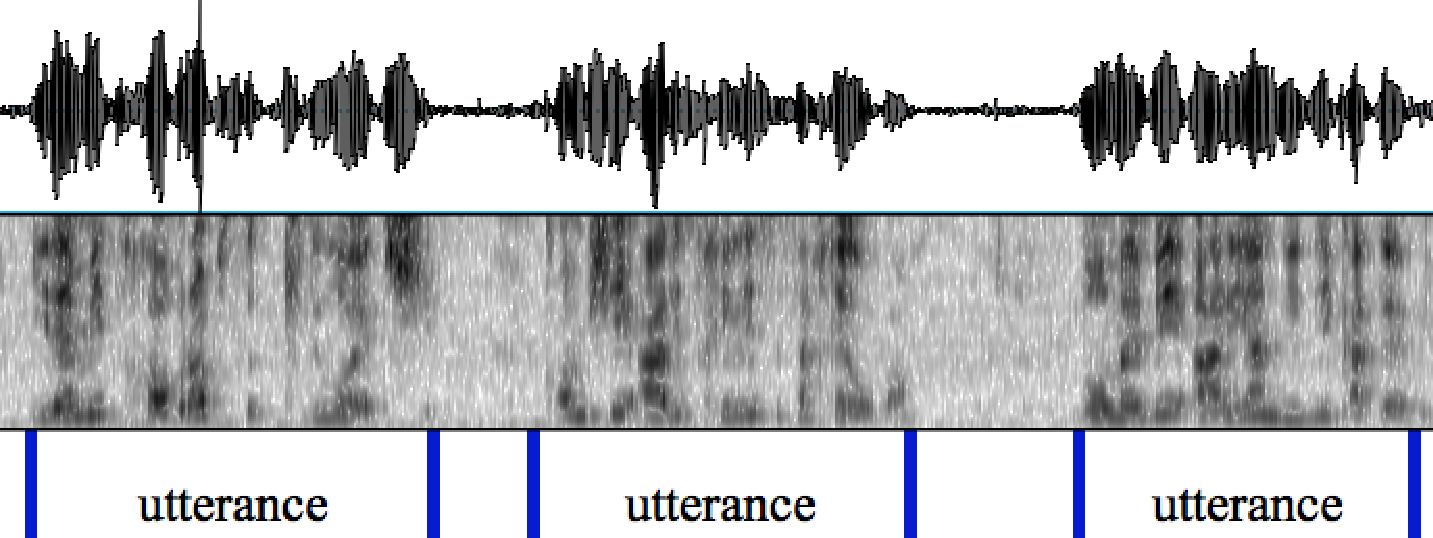
\includegraphics[width=3in]{images/utterance_extraction}
\caption{Screenshot of the utterance extraction process which converts any
audio/video into utterance intervals encoded either as \gls{json} or TextGrid using
the PraatTextGridJS library.}
\label{utterance_extraction_screenshot}
\end{center}
\end{figure}


\section{Using LingSync/OLD}\label{open-data}

% I commented out this paragraph to save space and because I didn't think it
% was contributing much beyond what we've already said.

%LingSync/OLD users are able to make subsets of their data stores publicly
%accessible while the language documentation project is active for the
%advancement of (at least) four distinct endeavours: 1) theoretical linguistic
%research, 2) the development of language learning tools for heritage and second
%language learners, 3) software development for low-resource languages, and 4)
%computational linguistic research on low-resource languages.

Current notable results of the LingSync/OLD project include Kartuli Glasses
for Facebook (a transliterator from the Latin alphabet to the Kartuli
alphabet),%
\footnote{Chrome Store
\url{https://chrome.google.com/webstore/detail/kartuli-glasses/ccmledaklimnhjchkcgideafpglhejja}} %
Georgian Together for Android (a language learning app),%
\footnote{Android Store
\url{https://play.google.com/store/apps/details?id=com.github.opensourcefieldlinguistics.fielddb.lessons.georgian}} %
and Kartuli Speech Recognizer for Android.%
\footnote{Android Store
\url{https://play.google.com/store/apps/details?id=com.github.opensourcefieldlinguistics.fielddb.speech.kartuli}} %
These apps were developed in collaboration with Kartuli speakers and Kartuli
software developers in Batumi, Georgia during the Spring 2014 semester.

%Readers interested in up-to-date examples and tutorials on how to use LingSync/OLD interfaces may consult YouTube and the project websites, \url{http://lingsync.org} and \url{http://onlinelinguisticdatabase.org}. 

Field linguist readers interested in a more detailed feature breakdown of
LingSync and the OLD are encouraged to consult \cite{lingsync:2012} and
\cite{dunham2014docs}, respectively. Those interested in developing tools
with language communities are encouraged to consult the LingSync WhitePaper
\S 7.2 \cite{LingSync:2012:WP} and readers interested in computational
linguistics research are encouraged to consult the LingSync WhitePaper \S
7.4 \cite{LingSync:2012:WP}.


\section{Conclusion}

In this paper we hope to have illuminated some of the complexity involved in
building software for endangered language documentation which has resulted in software
fragmentation. We have presented LingSync/OLD,  an open-ended plugin
architecture which puts Software Engineering best practices and our collective
experience in the language technology industry  to use to address this
fragmentation. The LingSync/OLD project has worked in an iterative fashion,
beginning with \glspl{ui} for field linguists in 2012-2013 and \glspl{ui} for 
community members, and software libraries and training for software
developers in 2013-2014. User studies and the dissemination of potentially
novel language documentation and/or computational linguistics contributions are
expected in 2014-2015 and in the future as the project continues to iterate.
For technical updates, interested readers may view the project's completed
milestones;%
\footnote{\url{https://github.com/FieldDB/FieldDB/issues/milestones?state=closed}} %
for user-facing updates, readers may visit LingSync.org and
OnlineLinguisticDatabase.org.


\section*{Acknowledgements}

We would like to express our deep thanks to Tobin Skinner, Elise McClay, Louisa
Bielig, MaryEllen Cathcart, Theresa Deering, Yuliya Manyakina, Gretchen
McCulloch, Hisako Noguchi, Brian Doherty, Gay Hazan, Oriana Kilbourn, Kim Dan
Nguyen, Rakshit Majithiya, Mietta Lennes, Nivja de Jong, Ton Wempe, Kyle
Gorman, Curtis Mesher, Beso Beridze, Tornike Lasuridze, Zviadi Beradze, Rezo
Turmanidze, Jason Smith, Martin Gausby, Pablo Duboue, Xianli Sun, James Crippen,
Michael McAuliffe as well as countless other linguistics students, computer
science students and open source software developers who directly or indirectly
helped build LingSync/OLD to what it is today and will be in the future. We
would like to thank the ComputEL workshop reviewers, LingSync/OLD users and
would-be users for providing feedback, suggestions, asking tough questions, and
sending bug reports, all of which have been instrumental to the project's
success and helped drive its development. We would like to thank Faryal
Abbassi, Farah Abbasi, Tamilla Paghava, Esma Chkhikvadze, Nina Gatenadze, and
Mari Mgeladze for their friendship, patience and for sharing their language
with us.  Finally, we would like to thank Jessica Coon, Alan Bale and Michael
Wagner for their guidance and challenging us to keep the user interfaces simple
and yet flexible, as well as SSHRC Connection Grant (\#611-2012-0001) and SSHRC
Standard Research Grant (\#410-2011-2401) which advocates open source
approaches to knowledge mobilization and partially funded the students who have
doubled as fieldwork research assistants and interns on the project. All errors
and oversights are naturally our own.


\bibliographystyle{acl}
\bibliography{bibliography}


\end{document}
